%%%%%%%%%%%%%%%%%%%%%%%%%%%%%%%%%%%%%%%%%
% a0poster Portrait Poster
% LaTeX Template
% Version 1.0 (22/06/13)
%
% The a0poster class was created by:
% Gerlinde Kettl and Matthias Weiser (tex@kettl.de)
% 
% This template has been downloaded from:
% http://www.LaTeXTemplates.com
%
% License:
% CC BY-NC-SA 3.0 (http://creativecommons.org/licenses/by-nc-sa/3.0/)
%
%%%%%%%%%%%%%%%%%%%%%%%%%%%%%%%%%%%%%%%%%

%----------------------------------------------------------------------------------------
%	PACKAGES AND OTHER DOCUMENT CONFIGURATIONS
%----------------------------------------------------------------------------------------

\documentclass[a0,portrait]{a0poster}
\usepackage[utf8]{inputenc}
\usepackage[francais]{babel}
\usepackage[T1]{fontenc}

\usepackage{multicol} % This is so we can have multiple columns of text side-by-side
\columnsep=100pt % This is the amount of white space between the columns in the poster
\columnseprule=3pt % This is the thickness of the black line between the columns in the poster

\usepackage[svgnames]{xcolor} % Specify colors by their 'svgnames', for a full list of all colors available see here: http://www.latextemplates.com/svgnames-colors

\usepackage{times} % Use the times font

\usepackage{graphicx} 
\usepackage{booktabs} % Top and bottom rules for table
\usepackage[font=large,labelfont=bf]{caption} % Required for specifying captions to tables and figures
\usepackage{amsfonts, amsmath, amsthm, amssymb} 
\usepackage{wrapfig} % Allows wrapping text around tables and figures
\usepackage{tikz}
% \usetikzlibrary{calc,trees,positioning,arrows,chains,shapes.geometric,%
% decorations.pathreplacing,decorations.pathmorphing,shapes,%
% matrix,shapes.symbols,plotmarks,decorations.markings,shadows}
\usepackage[most]{tcolorbox}
\usepackage{array}

\newcommand{\captioncolor}{\color{black}}
\newcommand{\equtext}[1]{\mbox{\small{#1}}}
\begin{document}
\large
%----------------------------------------------------------------------------------------
%	POSTER HEADER 
%----------------------------------------------------------------------------------------

% The header is divided into two boxes:
% The first is 75% wide and houses the title, subtitle, names, university/organization and contact information
% The second is 25% wide and houses a logo for your university/organization or a photo of you
% The widths of these boxes can be easily edited to accommodate your content as you see fit

\begin{minipage}[b]{0.75\linewidth}
\veryHuge \color{NavyBlue} \textbf{Stage de Recherche en Informatique (Sup\'e{}lec 2A)} \color{Black}\\
\Huge\textit{ Génération de signaux micro-Doppler par réseaux de neurone }\\[18mm]
\huge \textbf{Paul LE GRAND DES CLOIZEAUX}\\[0.5cm] 
\huge LRI, CentraleSupélec, Université Paris-Saclay
\end{minipage}
%
\begin{minipage}[b]{0.20\linewidth}

\includegraphics[width=\textwidth]{logo_lri.jpg}
\end{minipage}

%\vspace{1cm} % A bit of extra whitespace between the header and poster content

%----------------------------------------------------------------------------------------

\begin{multicols}{2} % This is how many columns your poster will be broken into, a portrait poster is generally split into 2 columns

%----------------------------------------------------------------------------------------
%	CONTEXTE
%----------------------------------------------------------------------------------------

\begin{tcolorbox}[colback=blue!5!lime,colframe=green!75!black,title={\section*{Contexte}}]
\textbf{\Large{Objectif: Classifier des profils micro-Doppler d'objets volants}}\\
Des profils micro-Doppler de drones et d'oiseaux ont été collectés par l'ONERA.
\begin{center}
    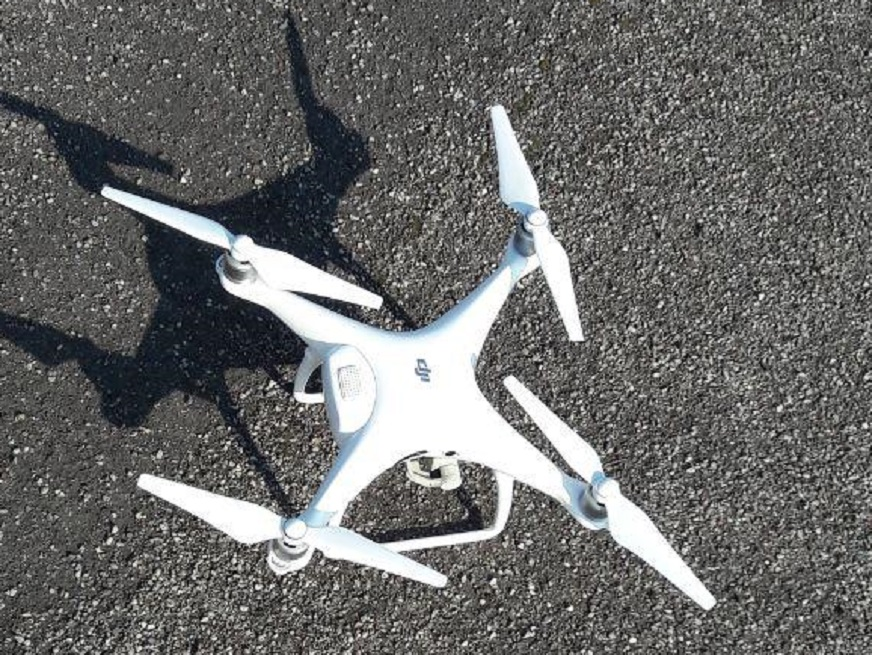
\includegraphics[width=0.19\textwidth]{./Phantom_version1.jpg}
    \captionof{figure}{Exemple de drone mesuré} 
\end{center}
\end{tcolorbox}
\bigskip

%----------------------------------------------------------------------------------------
%	Profils micro-Doppler
%----------------------------------------------------------------------------------------

\begin{tcolorbox}[colback=blue!5!white,colframe=blue!75!black,title={\section*{Profils micro-Doppler}}]
\textbf{Format: Spectrogramme en temps long}
\begin{center}
    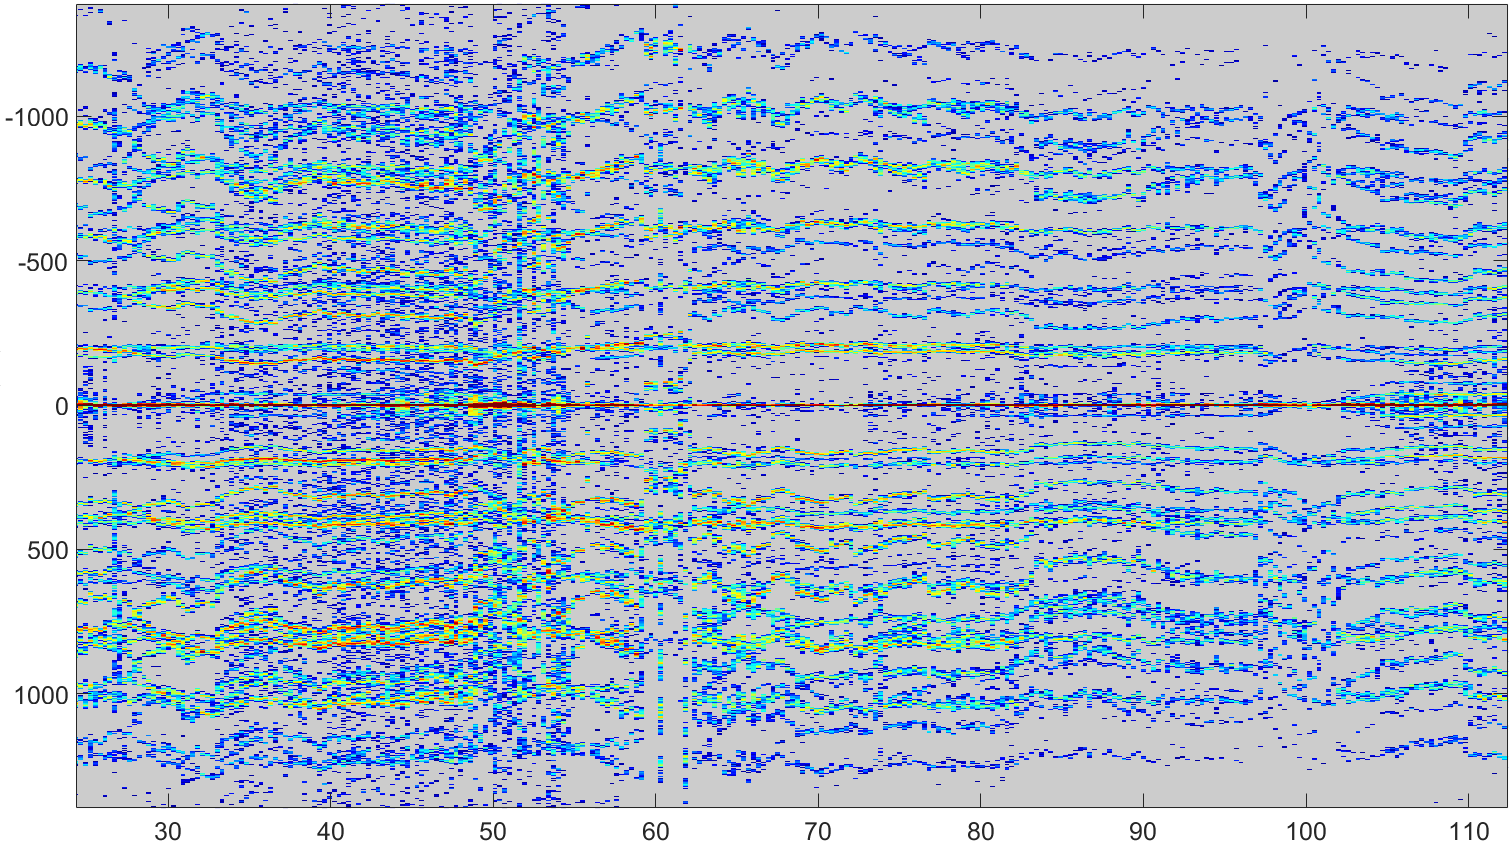
\includegraphics[width=0.9\textwidth]{./QD41.png}
    \captionof{figure}{\captioncolor Spectrogramme en temps long d'un drone}
    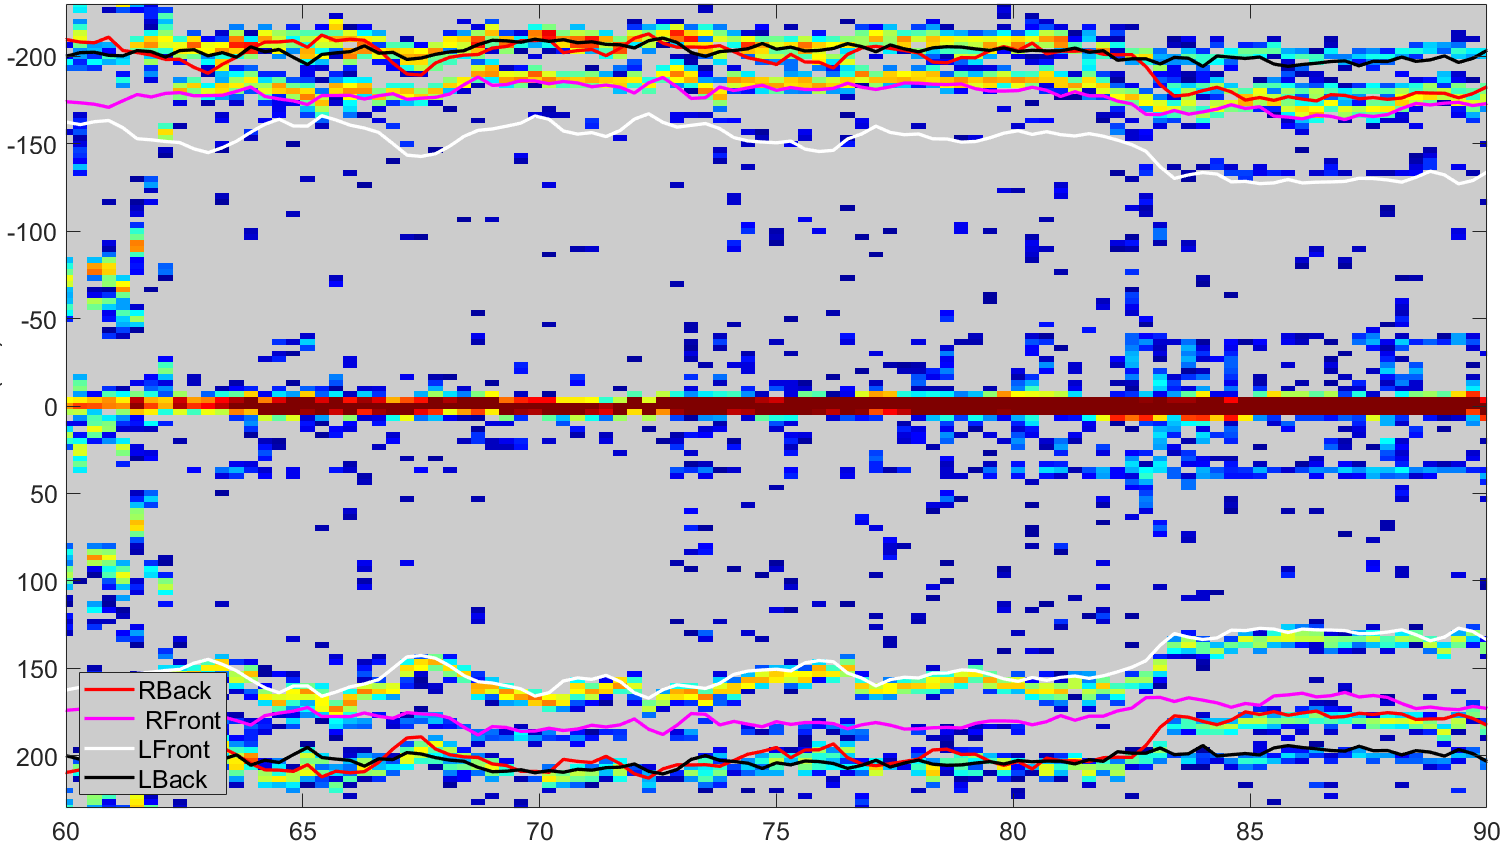
\includegraphics[width=0.9\textwidth]{./QD41_zoom.png}
    \captionof{figure}{\captioncolor Zoom - décalages de fréquences dus aux rotors}
\end{center}
\end{tcolorbox}
\bigskip

%----------------------------------------------------------------------------------------
%	Qu'est ce qu'un GAN?
%----------------------------------------------------------------------------------------
\begin{tcolorbox}[colback=blue!5!white,colframe=blue!75!black,title={\section*{Quantité de donnés insuffisantes}}]
\textbf{Problèmes}
\begin{itemize}
    \item Nombre faible de profils. \textbf{Quantité}
    \item Profils hautement corrélés. \textbf{Diversité}
\end{itemize}
\textbf{Solution proposée}\\
\textit{Data augmentation} par génération de profils micro-Doppler artificiels par réseaux de neurone (\textbf{GAN}).
\end{tcolorbox}
\bigskip

%----------------------------------------------------------------------------------------
%	Qu'est ce qu'un GAN?
%----------------------------------------------------------------------------------------

\begin{tcolorbox}[colback=blue!5!white,colframe=blue!75!black,title={\section*{Qu'est ce qu'un GAN (Generative Adversarial Network)?}}]
GAN : un réseau de neurone pour générer des données.
\begin{center}
    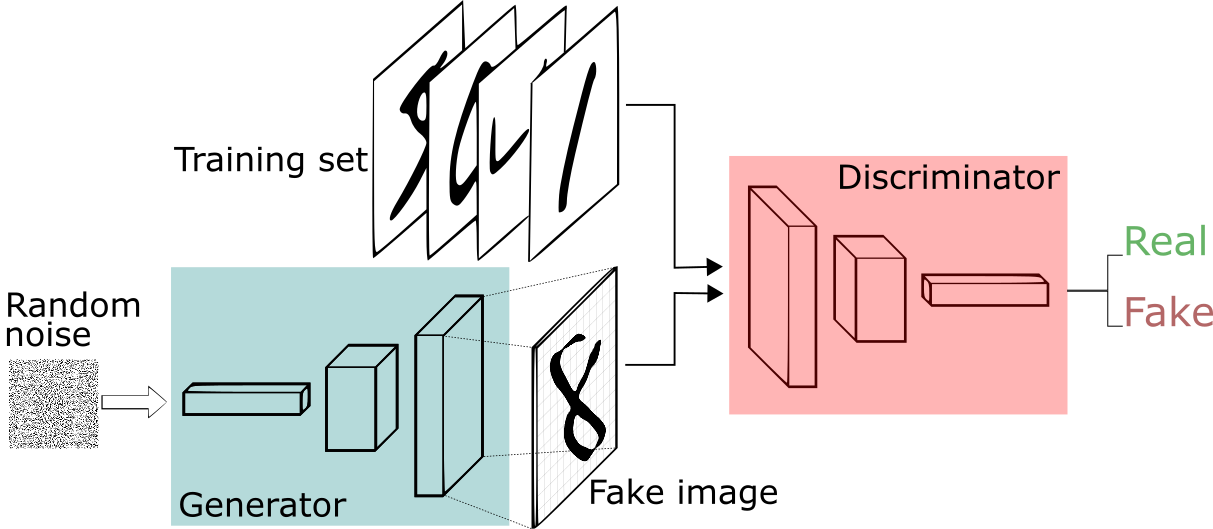
\includegraphics[width=0.7\textwidth]{./gan_schema}
    \captionof{figure}{\captioncolor Schéma d'un GAN basique} 
\end{center}
\subsection*{Fonctionnement}
Recherche d'un équilibre entre le \textbf{Générateur} et le \textbf{Discriminateur}.
\begin{itemize}
    \item \textbf{Générateur} essaye de tromper le \textbf{Discriminateur}
    \item \textbf{Discriminateur} essaye de démasquer le \textbf{Générateur}
\end{itemize}
Amélioration du \textbf{Générateur} par rétropropagation de l'erreur du \textbf{Discriminateur} sur l'image.
\end{tcolorbox}
%\bigskip

%----------------------------------------------------------------------------------------
%	Différents types de GAN
%----------------------------------------------------------------------------------------

\begin{tcolorbox}[colback=blue!5!white,colframe=blue!75!black,title={\section*{Différents types de GAN}}]
\textbf{Différentes architectures de réseau}\\
D discriminateur, G générateur, c labels, x données réelles, z vecteur de bruit
\begin{center}
\begin{minipage}{0.24\textwidth}
    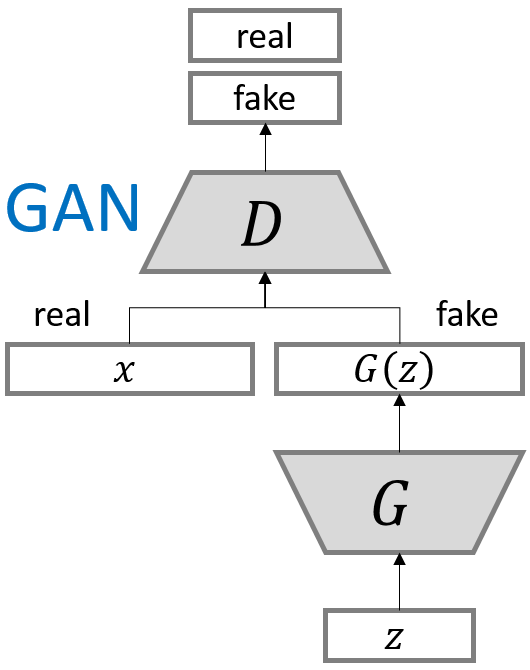
\includegraphics[width=1.0\textwidth]{./GAN_normal.png}
\end{minipage}
\begin{minipage}{0.31\textwidth}
    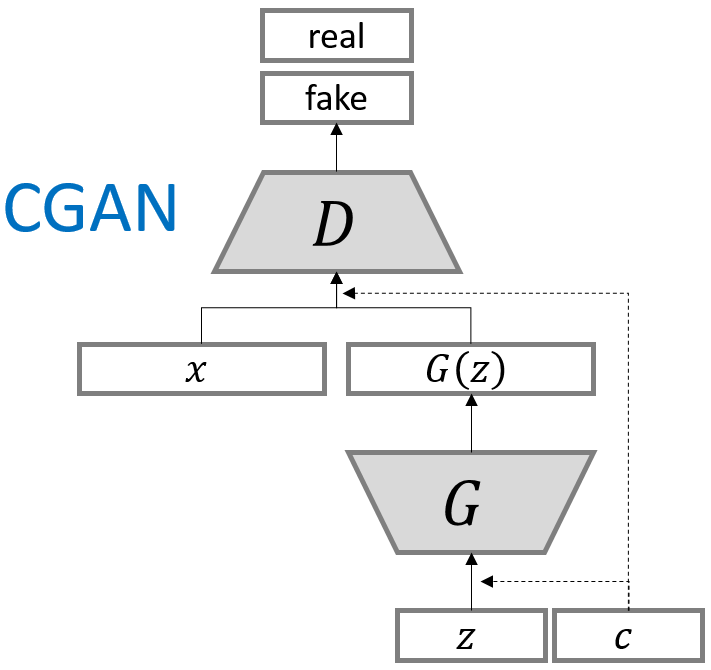
\includegraphics[width=1.0\textwidth]{./CGAN_structure.png}
\end{minipage}
\begin{minipage}{0.35\textwidth}
    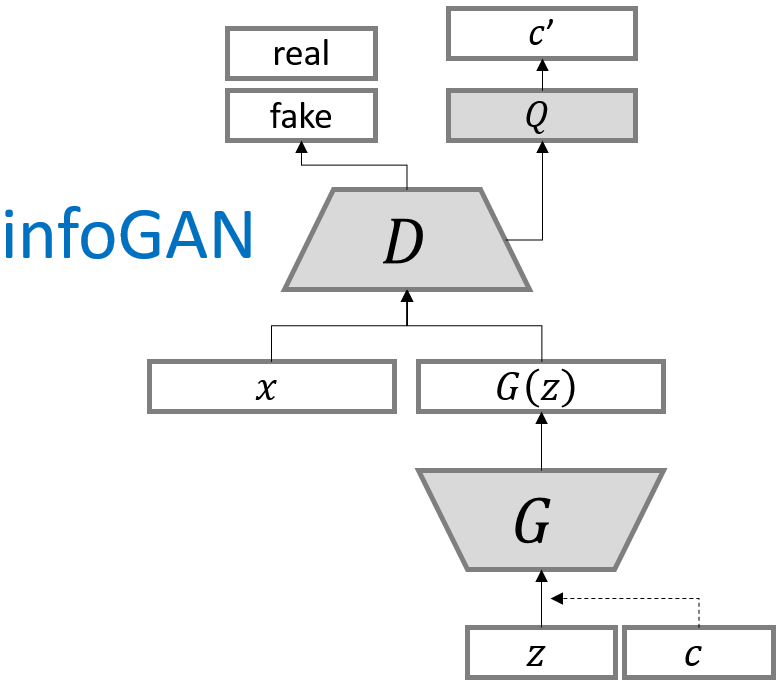
\includegraphics[width=1.0\textwidth]{./INFOGAN_structure.png}
\end{minipage}
\end{center}
\textbf{Différentes fonctions d'erreurs du Discriminateur}
\begin{itemize}
    \item Entropie croisée
    \item Distance de Wasserstein
\end{itemize}
\end{tcolorbox}
\bigskip
%----------------------------------------------------------------------------------------
%	Mesurer les performances d'un GAN?
%----------------------------------------------------------------------------------------

\begin{tcolorbox}[colback=blue!5!lime,colframe=green!75!black,title={\section*{Mesurer les performances d'un GAN?}}]
Comment mesurer la qualité des données générées par un GAN?
\begin{itemize}
    \item Pas possible d'évaluer le réseau sur une base de test.
    \item Évaluation humaine peu fiable, notamment pour les profils micro-Doppler.
\end{itemize}
\end{tcolorbox}
\bigskip

%----------------------------------------------------------------------------------------
%	FID
%----------------------------------------------------------------------------------------

\begin{tcolorbox}[colback=blue!5!white,colframe=blue!75!black,title={\section*{FID (Fréchet Inception Distance)}}]
\textbf{Evaluation d'une distance entre deux ensembles d'images}\\
\textbf{InceptionV3}, réseau de neurone à convolution entraîné sut ImageNet est utilisé pour extraire des motifs de l'image.\\
Comparaison des statistiques de sorti l'avant-dernière couche du réseau.
\begin{center}
$X_{\equtext{real}}=\mathcal{N}(\mu_{\equtext{real}}, \Sigma_{\equtext{real}}), X_{\equtext{generated}}=\mathcal{N}(\mu_{\equtext{generated}}, \Sigma_{\equtext{generated}})$
$FID = ||\mu_{\equtext{real}} - \mu_{\equtext{generated}}||^2 + Tr(\Sigma_{\equtext{real}} + \Sigma_{\equtext{generated}}  - (\Sigma_{\equtext{real}} \Sigma_{\equtext{genrated}})^{1/2})$
\end{center}
\end{tcolorbox}
\bigskip

%----------------------------------------------------------------------------------------
%	Résultats
%----------------------------------------------------------------------------------------

\begin{tcolorbox}[colback=blue!5!white,colframe=blue!75!black,title,title={\section*{Résultats}}]
% \begin{minipage}{0.5\textwidth}
    \begin{center}
        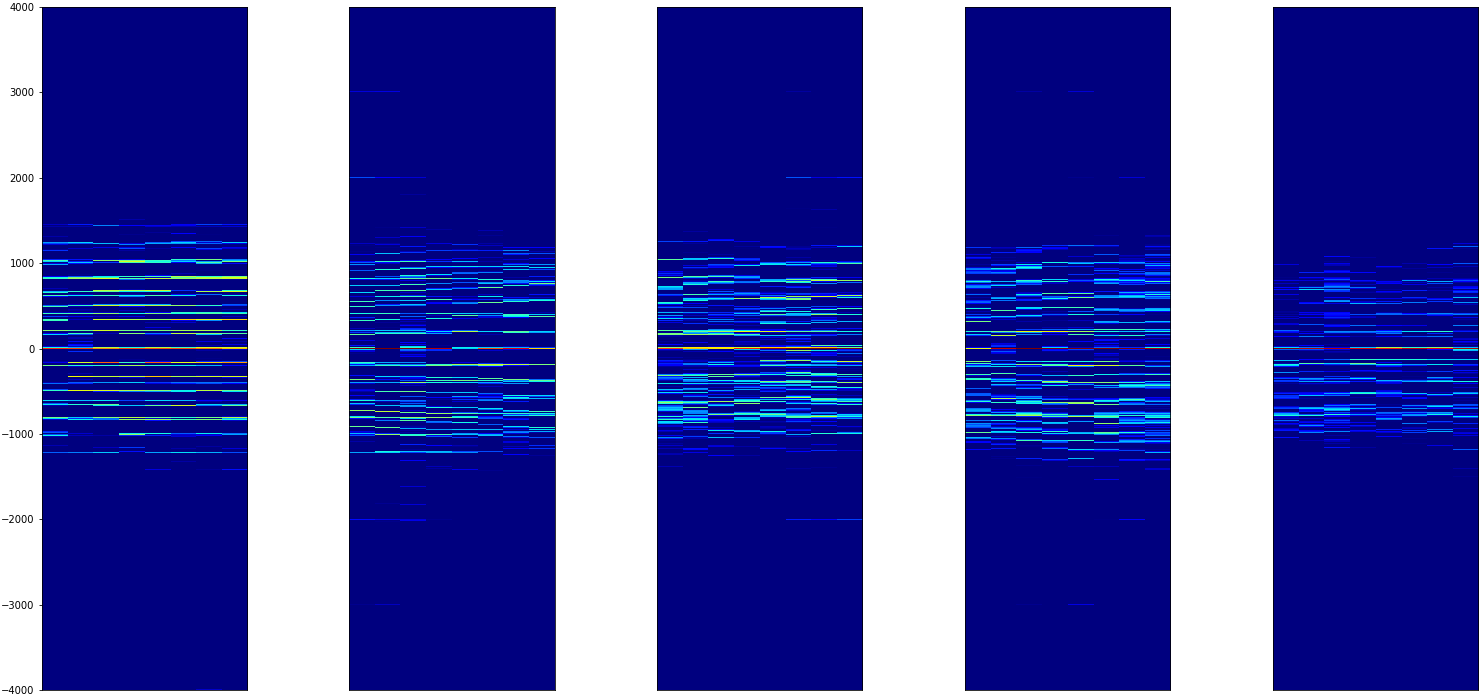
\includegraphics[width=\textwidth]{./profils_reels.png}
    \end{center}
    \captionof{figure}{Profils réels}
% \end{minipage}
% \begin{minipage}{0.5\textwidth}
    \begin{center}
        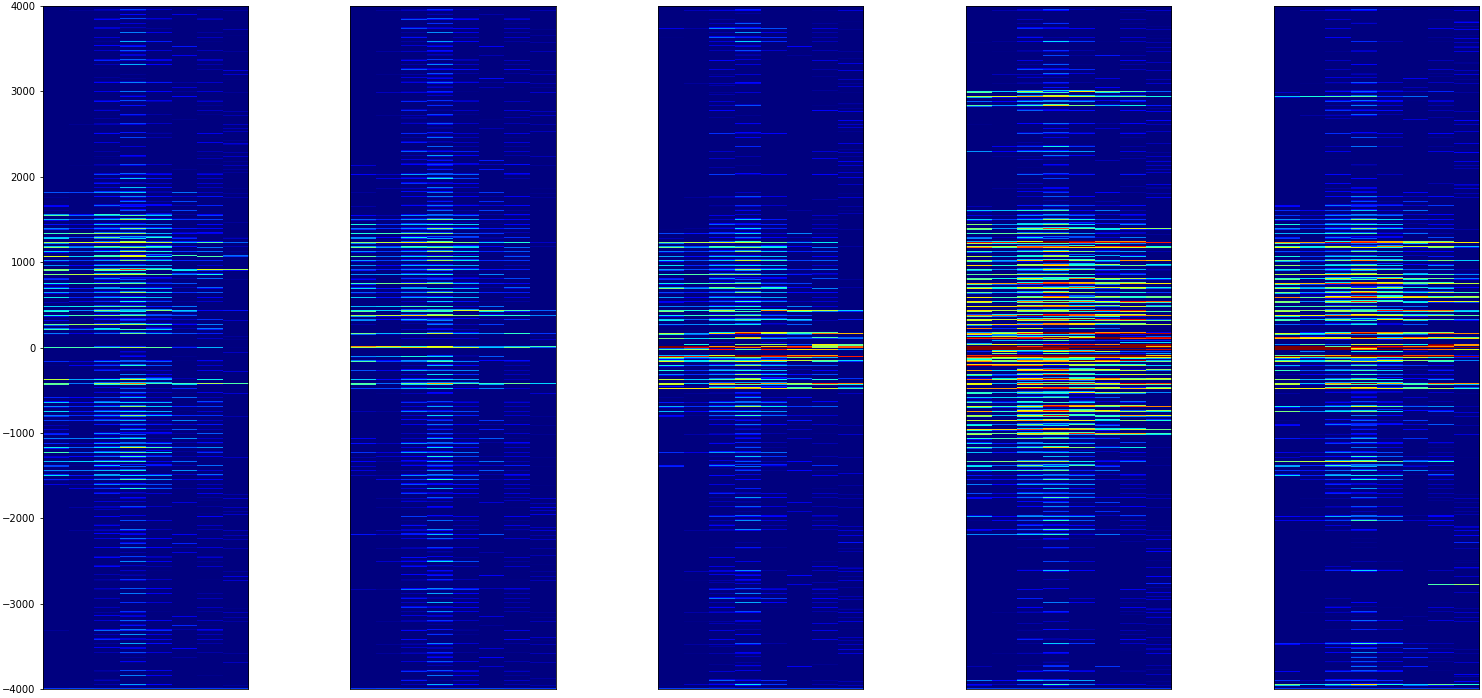
\includegraphics[width=\textwidth]{./profils_generes.png}
    \end{center}
    \captionof{figure}{Profils générés}
% \end{minipage}
\end{tcolorbox}
\bigskip

%----------------------------------------------------------------------------------------
%	PERSPECTIVES
%----------------------------------------------------------------------------------------

\begin{tcolorbox}[colback=red!5!orange,colframe=red!75!black,title={\section*{Perspectives}}]
Les signaux générés ne sont pas de très bonne qualité.\\
\textbf{Améliorations}
\begin{itemize}
    \item \textit{Parameters tunning}
    \item GAN \textit{image-to-image}, tel que \textbf{CycleGAN}, à partir de profils micro-Doppler simulés. Permettrait de générer des profils de drones non présent dans la base de donnée.
    \item GAN plus avancés (par exemple \textbf{StyleGAN})
\end{itemize}
\end{tcolorbox}
\end{multicols}
\end{document}
